%\graphicspath{{/media/data/Work/cnstellate/DS_ClickRecovery/}{/media/data/Work/Responses/}{../figures/}{./gfx/}}

\section[DS Cell Model]{D~Stellate Cell Model: Optimisation using click recovery responses}   \label{sec:d-stellate-cell-model}

\subsection{Introduction}

This section shows the GABAergic input and intrinsic cell properties influence the behaviour of D~stellate cells.
In the mammalian \VCN~have a wide ranging influence on the primary cells of the \VCN, especially stellate and bushy neurons \citep{RhodeSmithEtAl:1983}, the ipsilateral \DCN~(type II and type IV \EIRA~units) and the contralateral \CN~\citep{NeedhamPaolini:2007}.

% \smallskip{}

% Large multipolar or stellate cells in the \VCN~have been shown to have 3-4
% long dendrites stretching 200 microns (or one third of the \VCN) and their
% axonal collaterals cover the same region in the \VCN, almost one half of the
% \DCN, and are one source of the commissural projection to the contralateral
% cochlear nucleus \citep{NeedhamPaolini:2007}.
%%%%%%%%%%%%%%%%%%% Copied from original jneurometh article

\DS~cells are large multipolar neurons in the \VCN~and have an \OnC~\PSTH~to tones and noise \citep{SmithRhode:1989,NeedhamPaolini:2006}.
They typically have 3-4 long dendrites stretching 200 microns (or one third of the \VCN) and their axonal collaterals cover the same region in the \VCN, almost one half of the \DCN, and are one source of the commissural projection to the contralateral cochlear nucleus \citep{Cant:1992,Cant:1981,SchofieldCant:1996,CantBenson:2003,NeedhamPaolini:2007,PaoliniClark:1999}.
Intracellular responses to sounds indicate the bandwidth of inputs to \DS~neurons typically ranges from two octaves below \CF~to one octave above \CF~\citep{PalmerJiangEtAl:1996,JiangPalmerEtAl:1996,PaoliniClark:1999}.
\DS~cell axon terminals contain the inhibitory neurotransmitter glycine and synapse widely in the \VCN~and \DCN.
They also send a commissural projection to the contralateral cochlear nucleus that mediates fast inhibition between the nuclei \citep{NeedhamPaolini:2003,NeedhamPaolini:2006,Oertel:1997}.

% \smallskip{}

Post-onset GABAergic inhibition in \DS~cells is a major influence on the \PSTH~of \OnC~neurons \citep{FerragamoGoldingEtAl:1998a,EvansZhao:1998}.
Latency of excitation to auditory nerve shocks suggests Golgi cells are activated by type II \ANFs~and low spontaneous rate type I~\ANFs~\citep{BensonBerglundEtAl:1996,FerragamoGoldingEtAl:1998}.
Therefore, type II and \LSR~type I \ANFs~could be involved in gain control through GABAergic modulation of activity in the \VCN.

% \smallskip{}

% \yellownote{Discuss AM coding by \DS~cells} \GABA~blockers in the \VCN~has the
% effects of changing the behaviour in the response to AM in the IC
% \citep{CasparyPalombiEtAl:2002}.  AM coding effects of GABA in the Chinchilla
% \CN~\citep{BackoffShadduckEtAl:1999}. \citep{CasparyBackoffEtAl:1994} Caspary
% and colleagues worked on the effects of \GABA~in in the \VCN.

% Zhang and Winter looked at the response area of \VCN~onset units to determine
% \GABA~{on\slash off} freq.

% Smith and Rhode, Smith and others looked at OnC response area and two-tone


\subsection{Implementation}


% 2.5. Data analysis 
% Data were collected as spike times with a resolution of 10
% μs and analyzed off-line on a micro-VAX 3100 (Digital). Response histograms
% were plotted and analyzed using a windowing technique in which spike counts
% were taken over brief time windows of identical duration for the masker and
% probe components (Fig. 1B). Using the control conditions, counting windows
% were determined individually for each unit but ranged between 1 and 4 ms based
% on the control response to the masker alone and the probe alone. To assess
% response variability over time, repeated unmasked controls for both the masker
% (masker alone, Ma) and probe (probe alone, Pa) were obtained during the
% pre-drug, drug, and post-drug recovery conditions. Drug doses were determined
% empirically as the lowest dose that elicited a reproducible and reversible
% effect. To allow normalization of the masked probe response obtained in the
% paired-click paradigm to the unmasked response obtained when the probe was
% presented alone, identical measurement windows were used in the control and
% drug conditions for a given unit. The suppression recovery functions for each
% unit were normalized by taking the ratio Pm/Pa where Pm is the masked probe
% spike count and Pa is the unmasked response to the probe (Fig. 1C).



Key elements in designing D~stellate cell model are shown in the Nordlie table~\ref{tab:DScellModelSummary}A.
A type I-II single compartment neuron by \citet{RothmanManis:2003b} has the characteristics of a onset chopper unit and has previously been used to simulate a \DS~cell model.
The choice of having a large multipolar neuron without dendrites was based on computational efficiency and ensuring that the model fit within the criteria for DS cells.
The electrotonic dendrites of \DS~cells mean that the filtering in \DS~cells primarily controls the height of excitatory {\PSPs} reaching the soma \citep{WhiteYoungEtAl:1994}, hence a single compartment with graded weights should suffice.


The synaptic connections onto the D~stellate cell model, shown in table~\ref{tab:DScellModelSummary}C, are simplified to afferent ANF inputs and intra-nuclear col-localised GABAergic input from Golgi cells.
The \ANF~spread onto \DS~cells is well documented \citep{PaoliniClark:1999,ArnottWallaceEtAl:2004,PalmerWallaceEtAl:2003,JiangPalmerEtAl:1996,PalmerJiangEtAl:1996}, hence a decision made to fix this parameter due to the large computational task of calculating an optimisation routine for \ANFDS bandwidth.
The spread \ANF~to \DS~cells (\sANFDSh,\sANFDSl) is set so that 2 octaves below and 1 octave above \CF~are within 2 standard deviations \citep{PaoliniClark:1999}.


The physiological effect of GABAergic inputs onto onset choppers is primarily on CF~\citep{CasparyHaveyEtAl:1979,PalombiCaspary:1992,CasparyBackoffEtAl:1994,CasparyPalombi:1993,CasparyPalombiEtAl:1993}, but the bandwidth is difficult to ascertain.
The dendrites of D~stellate cells cover one third of the nucleus (approximately 3 octaves of tonotopic frequencies) and occasionally project into the \GCD~\citep{ArnottWallaceEtAl:2004}.
Golgi cells' axonal collaterals are confined to 200 microns in the \GCD~and \ANF~tonotopic organisation in the \GCD~is less defined.
The \GLGDS~spread is set to 2 channels with zero offset, which corresponds to a \DS~cell selecting from approximately 5 nearest Golgi cells.

\begin{figure}[htb]
  \centering
%  \resizebox{0.8\textwidth}{!}{}
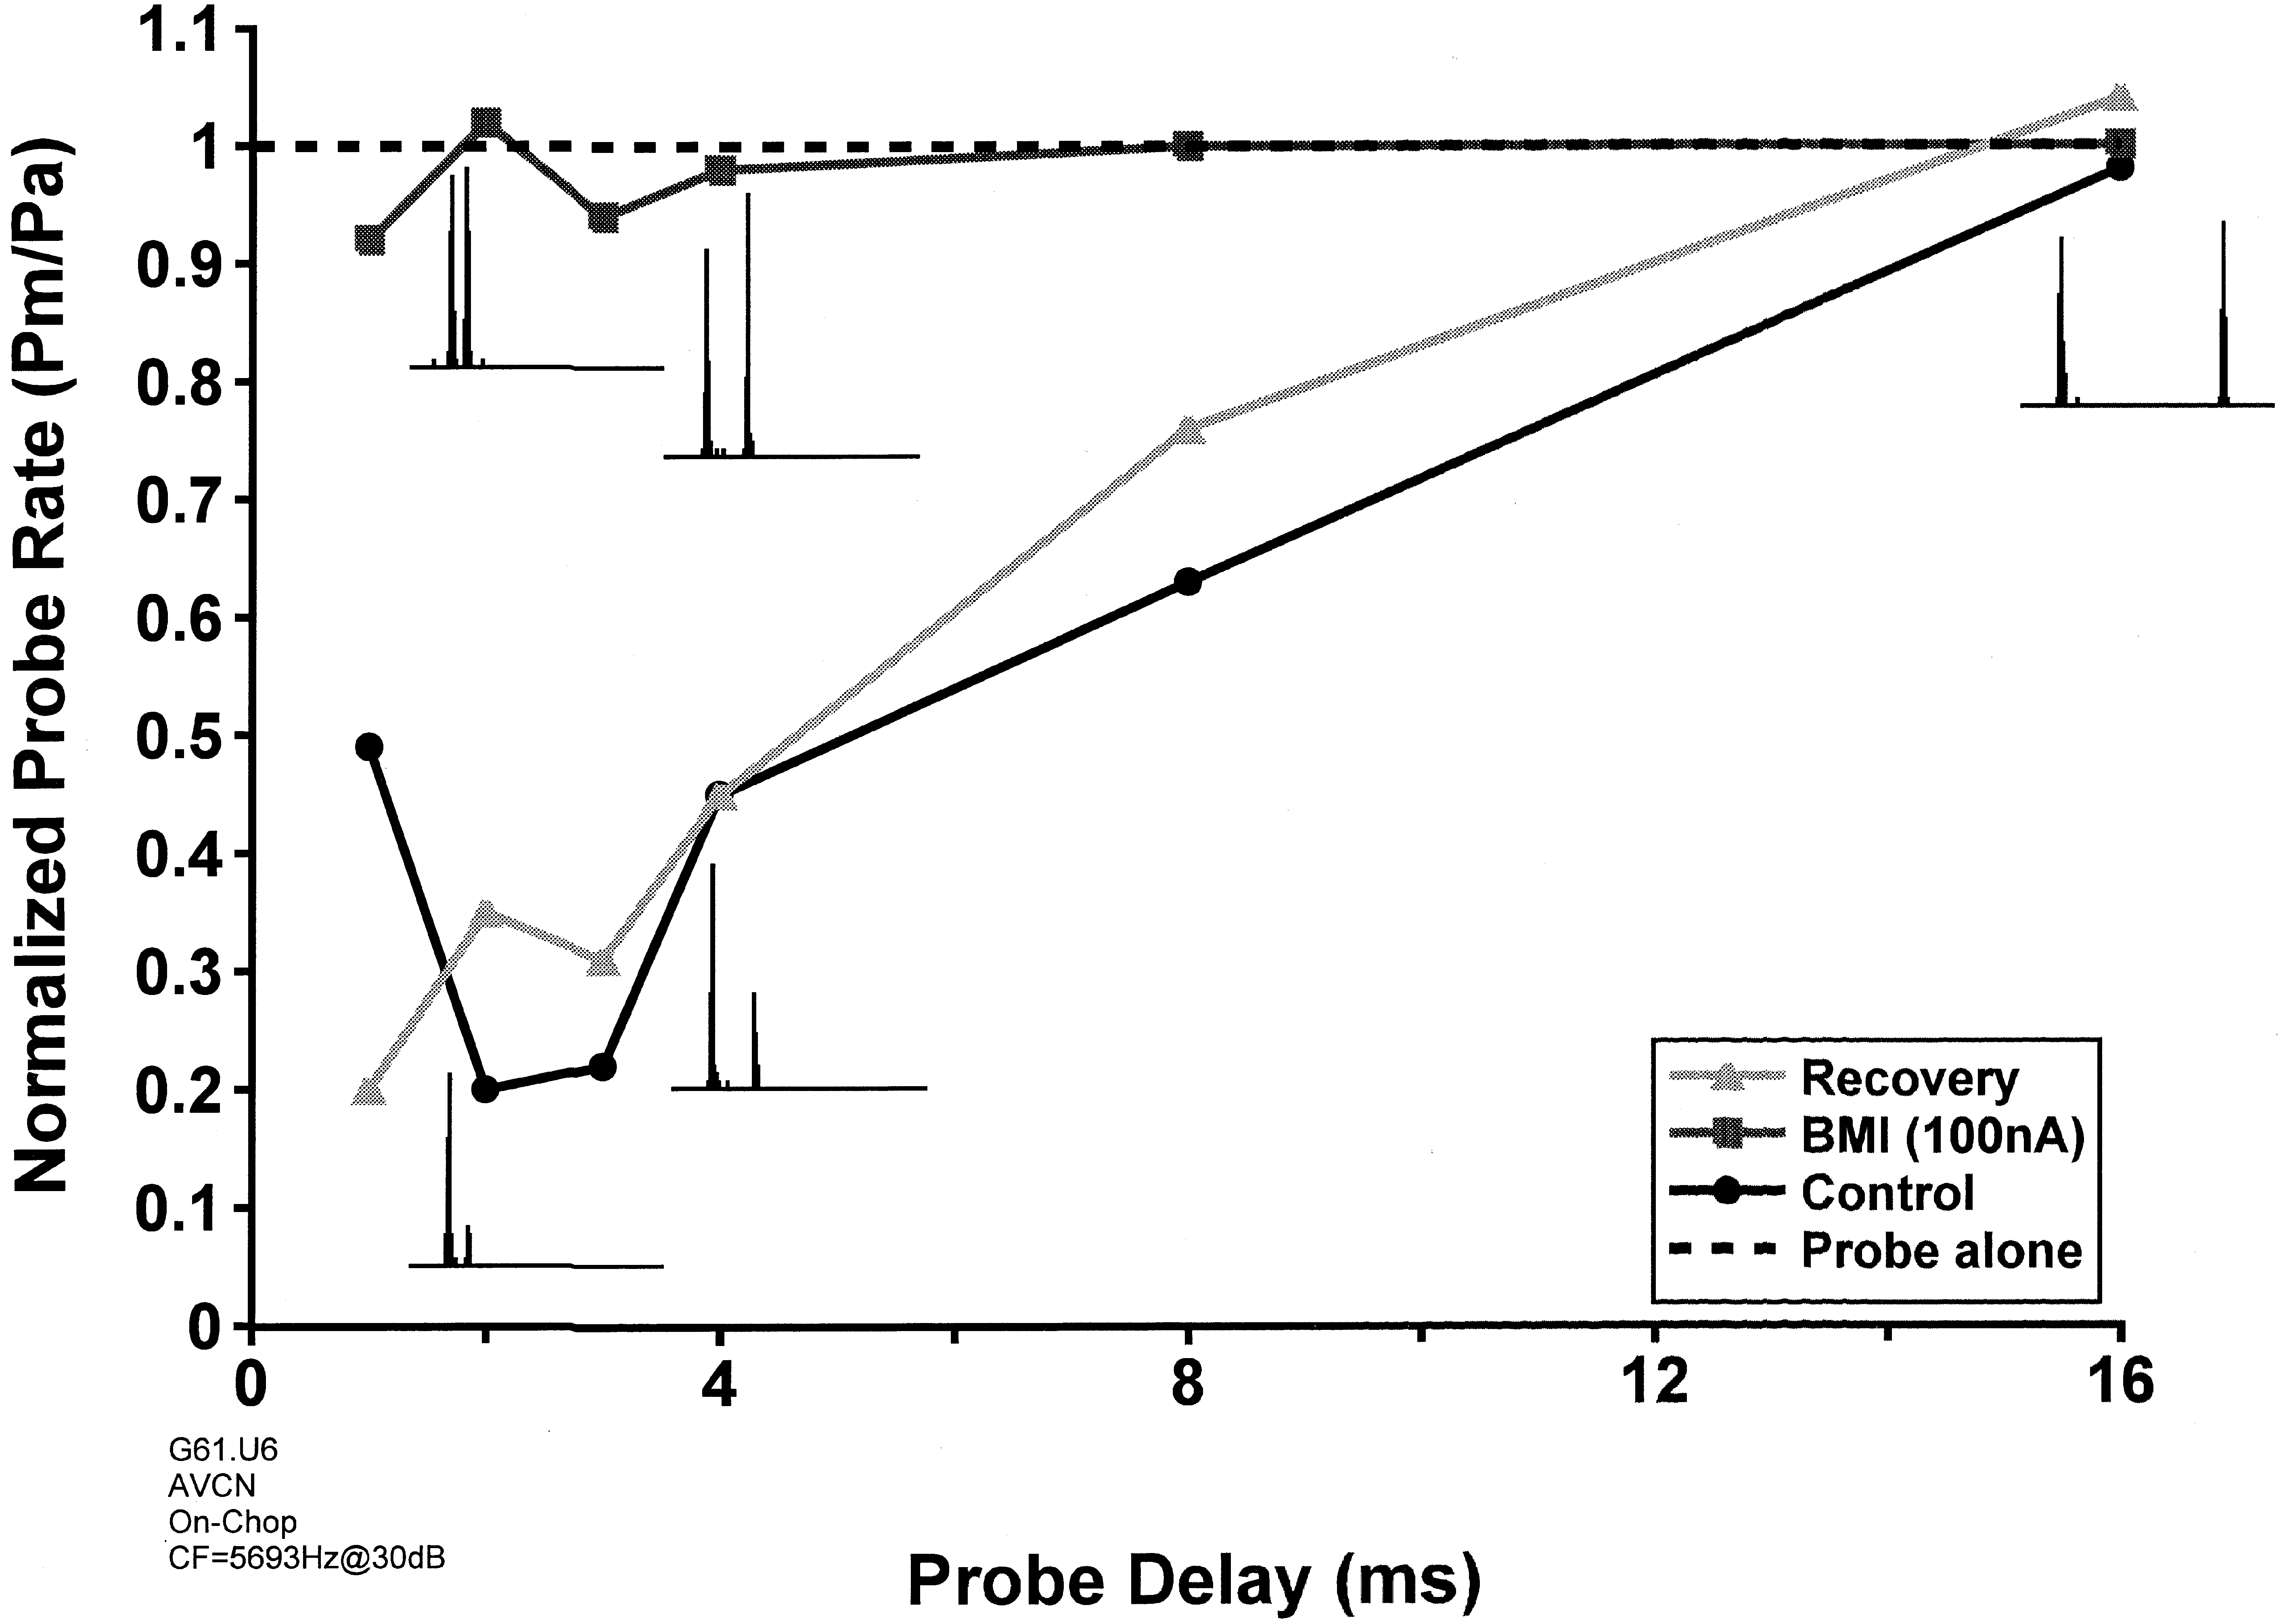
\includegraphics[keepaspectratio,width=0.8\textwidth]{gfx/Backoff+Palombi-Fig3}
  \caption{Experimental data showing click recovery in onset choppers}\label{fig:BackoffPalombi}
\end{figure}

Fixed parameters included  the number of Golgi cells to \DS~cells ($\nGLGDS = 25$), the spread of \ANFs~to \DS~cells $\ANFDS$, and the extra delay from the auditory nerve.

The first spike latency in high \CF \DS~cells ($2.8 \pm 0.09$ ms) is precise and faster than other stellate neurons in the VCN \citep{RhodeSmith:1986}.

The addition of 0.5~ms to \ANFDS~connections is a combination of conductance and synaptic delay.

The effect of Golgi cells on \DS~is delayed by the extra 0.7~ms delay from \ANF~to Golgi, plus the slow peak of \GABAa~inhibition.
\yellownote{fix this paragraph}


% \smallskip{}
%\subsubsection{Optimisation routine}
\subsection{Results}    \label{sec:DS:results}

Optimisation parameters for \GLGDS~are optimised based on experimental click recovery data from \citep{BackoffPalombiEtAl:1997}, as shown in Figure~\ref{fig:BackoffPalombi}.
The input stimulus presented a series of masker-probe clicks, with intervals of 2, 3, 4, 8, and 16 ms, separated by 50 ms.
Although the experimental stimuli was presented every 250 ms, the optimisation stimulus needs to be computationally efficient so the separation was shortened and the sequence reordered to obtain the best click recovery response in the \DS~and Golgi cells.
The stimulus was repeated 25 times and a PSTH was produced from the DS cells' spikes.
Spike counts for 2 ms after the probe and masker click were selected (accounting for the the minimum first spike latency for the unit) to calculate a recovery ratio.
The \DS~cell optimisation function calculates the mean squared error between the test model and the experimental data recovery ratios to 5 click pairs.


The six parameters to be fit by the routine are the weights of \GLG\@, \HSR\@, and \LSR~synapses on \DS, the \GABAa synapse rise constant, the \GABAa synapse decay constant, and the \DS~cell maximum leak conductance.
Initial optimisation procedures were not successful at constraining the short delay recovery responses (2,3,4 ms), hence the \DS~cell leak %and \KLT~conductance parameters  parameter were included in the optimised parameters to allow cell's input resistance behaviour to fit fast acting behaviour in the cell.

The unit used in the optimisation has a \CF~of 5.8~kHz (equivalent to channel no. 50 in the CN network with 100 channels from 0.2 to 30~kHz).

\begin{figure}[htb]
\centering
%\resizebox{0.6\textwidth}{!}{}
\includegraphics[keepaspectratio,width=0.6\textwidth]{DS_ClickRecovery/ANinput}
%   \subfloat[D~stellate cell]{
%\includegraphics[width=0.4\textwidth]{DS_ClickRecovery_DSpsth}% \label{fig:DSClickRecoveryPSTH}
%}\quad%   \subfloat[Golgi cell]{
  %\includegraphics[width=0.4\textwidth]{DS_ClickRecovery_Gpsth}%\label{fig:GClickRecoveryPSTH}%}
\caption[Click recovery stimulus]{Click stimulus and PSTH responses of an HSR fibre, a GLG unit, and a DS unit from the click recovery stimulus used in the optimisation. }\label{fig:ClickExamples}
\end{figure}


% \smallskip{}

% \noindent\begin{tabularx}{\textwidth}{|l|X|}\hline %{\textwidth}
% \hdr{2}{D}{Results} \\\hline
% \end{minipage}}\\\hline
% \textbf{Error} & 0.006671    unweighted (MSE of recovery spike rate / mask rate)\\\hline
% & 0.01447    final result (MSE of recovery spike rate / mask rate)\\\hline
% \end{tabularx}

{\small% - E ------------------------------------------------------------------------------
\noindent
\begin{tabularx}{\textwidth}{|X|c|c|c|}\hline %{\textwidth}
\hdr{4}{E}{Optimisation} \\ \hline
        \textbf{Parameters}          &   \textbf{Name}  & \textbf{Range} & \textbf{Best Values} \\\hline
      Weight of \GLG~on \DS~(nS)       &     \wGLGDS      & [0.01,50] & 0.532 \\	\hline
    Weight of \HSR~syn on \DS~(nS)     &     \wHSRDS      & [0.01,50] & 0.16 \\ \hline
   Weight of \LSR~syn on \DS~(nS)     &     \wLSRDS      &   [0.01,50] & 13.1 \\	    \hline
 \GABAa synapse rise constant  (ms)  &  $\tau_{GABA1}$  & [0.01,10.0] & 5.432\\	     \hline
 \GABAa synapse decay constant (ms)  &  $\tau_{GABA2}$  & [0.1,50.0] & 0.262\\	    \hline
DS cell leak conductance (mS cm$^{-2}$) & \gleak &  [1e-5,0.05]   & 0.0163 \\ \hline
\end{tabularx}
\vspace{2ex}
}


The optimisation parameters show a clear favouritism toward the \LSR~input rather than the \HSR~input to \DS~units.
While this may not seem ideal for fast coincidence detection, the large number of \HSR~synapses makes up for the small weight that was obtained in the optimisation.

\begin{figure}[htb]
\centering
%\resizebox{0.9\textwidth}{!}{\includegraphics{NoFigure}}
%\resizebox{0.8\textwidth}{!}{}
\includegraphics[height=0.8\textwidth,keepaspectratio,angle=-90]{DS_ClickRecovery/DS_ClickRecovery_result}
\caption[Click recovery optimisation results in DS cell model]{%
Optimisation results of click recovery behaviour in DS cell model (CF 5.8~kHz).
The optimal response (blue circle) is obtained from Fig.~3 in \citet{BackoffPalombiEtAl:1997}, representing the click recovery response of an OnC unit (CF 5.8~kHz).
Best result (green triangles).   } \label{fig:DS_ClickRecovery_result}
\end{figure}



% \begin{figure}
% \includegraphics[width=0.5\textwidth]{DS_ClickRecovery_OptVars.eps}\\
% % \includegraphics[width=0.5\textwidth]{DS_ClickRecovery_Output.eps \label{Ch3:fig:DSClickRecoveryOutput}}
%   \caption{Final Output Data of the D~stellate Click Recovery optimisation }
% \end{figure}
% \begin{figure}
% \includegraphics[keepaspectratio=true,width=0.8\textwidth]{DS_ClickRecovery_Example1.eps}\\
% \includegraphics[keepaspectratio=true,width=0.8\textwidth]{DS_ClickRecovery_Example10.eps}\\
% \includegraphics[keepaspectratio=true,width=0.8\textwidth]{DS_ClickRecovery_Example13.eps}\\
% \includegraphics[keepaspectratio=true,width=0.8\textwidth]{DS_ClickRecovery_Example19.eps}\\
%   \caption{Click Recovery optimisation functions}
% \end{figure}


% \begin{figure}
% \includegraphics[keepaspectratio=true,angle=-90,width=0.8\textwidth]{DS_ClickRecovery_result1.eps}\\
% \end{figure}


% \begin{figure}
% \includegraphics[keepaspectratio=true,angle=-90,width=0.8\textwidth]{DS_ClickRecovery_result2.eps}\\
%   \caption{Click Recovery optimisation }
% \end{figure}


% \begin{figure}
%   \begin{center}
% \includegraphics[keepaspectratio=true]{DS_ClickRecovery_handtuned.eps}\\
% \includegraphics[keepaspectratio=true,angle=-90,width=0.8\textwidth]{DS_ClickRecovery_result_handtuned.eps}
%     \caption{Handtuned}
%     \label{hantuned}
%   \end{center}
% \end{figure}

% \begin{figure}
%   \begin{center}
% % \includegraphics[keepaspectratio=true]{DS_ClickRecovery_handtuned.eps}\\
% \includegraphics[keepaspectratio=true,angle=-90,width=0.8\textwidth]{gfx/DS_ClickRecovery_result_unweighted_8.eps}\\
% \includegraphics[keepaspectratio=true,angle=-90,width=0.8\textwidth]{gfx/DS_ClickRecovery_result_weighted_0.eps}
%     \caption{Handtuned}
%     \label{hantuned}
%   \end{center}
% \end{figure}

\clearpage
% \newpage
\subsection{Verification}    \label{sec:DS:verification}

\yellownote{Small presentation of PSTH, RL, NRL, MRC and RA. Leave AM responses till next chapter}

\begin{figure}[htb]
%\centering\hspace{0.5cm}
\figfont{A}\hspace{0.5\textwidth}\figfont{B}\hfill\\
%\resizebox{0.95\textwidth}{!}{
\includegraphics[keepaspectratio=true,width=0.48\textwidth]{ResponsesNoComp/DS_ratelevel_combined.eps}%
\includegraphics[keepaspectratio=true,width=0.48\textwidth]{ResponsesNoComp/RateLevel/psthsingle90.2.eps}\\
%}\\\hspace{0.5cm}
\figfont{C}\hspace{0.5\textwidth}\figfont{D}\hfill\\
%  \resizebox{0.95\textwidth}{!}{%
\includegraphics[keepaspectratio=true,width=0.48\textwidth]{ResponsesNoComp/RateLevel/response_area.2.eps}%
\includegraphics[keepaspectratio=true,width=0.48\textwidth]{ResponsesNoComp/MaskedResponseCurve3/15/DS_masked.eps}\\
%}\\
% }}
%\resizebox{0.45\textwidth}{!}{\includegraphics{ResponsesNoComp/RateLevel/psthsingle90.3.eps}}\\
%\resizebox{0.45\textwidth}{!}{\includegraphics{ResponsesNoComp/RateLevel/psthsingle50.3.eps}}\\
\caption[Optimised DS cell model responses]{Response of optimised Golgi cell model at the centre of the network (CF=5.8~kHz). A. Rate level responses to tone, noise and tone plus noise. B. PSTH at 90 dB~SPL.  C. Response area equivalent using all DS units in the network. D. Masked response across the CF of the central unit (15 dB noise).} \label{fig:DS_verification}
\end{figure}


% \subsection{Tone Responses}
% \begin{figure}[h!]
%   \centering\resizebox{\textwidth}{!}{%
%   \includegraphics{RateLevel/psthsingle90.2.eps}%
%   \includegraphics{RateLevel/DS_ratelevel.eps}}
% \end{figure}
% \begin{figure}[h!]
%   \centering\resizebox{\textwidth}{!}{%
%   \includegraphics{RateLevel/response_area.2.eps}%
%   \includegraphics{RateLevel/response_area_log2.2.eps}}
% \end{figure}
% \begin{figure}[h!]
%   \centering\resizebox{\textwidth}{!}{%
% %   \includegraphics{RateLevel/response_area.2.eps}
%   \includegraphics{RateLevel/psthall90.2.eps}%
%   \includegraphics{RateLevel/psthVlevel.2.eps}}
% \end{figure}


% \clearpage
% \subsection{Noise Responses}
% \begin{figure}[h!]
%   \centering\resizebox{\textwidth}{!}{%
%   \includegraphics{NoiseRateLevel/psthsingle120.2.eps}%
%   \includegraphics{NoiseRateLevel/DS_ratelevel.eps}}
% \end{figure}
% \begin{figure}[h!]
%   \centering\resizebox{\textwidth}{!}{%
%   \includegraphics{NoiseRateLevel/response_area.2.eps}%
%   \includegraphics{NoiseRateLevel/response_area_log2.2.eps}}
% \end{figure}
% \begin{figure}[h!]
%   \centering\resizebox{\textwidth}{!}{%
% %   \includegraphics{RateLevel/response_area.2.eps}
%   \includegraphics{NoiseRateLevel/psthall90.2.eps}%
%   \includegraphics{NoiseRateLevel/psthVlevel.2.eps}}
% \end{figure}


% \clearpage
% \subsection{Masked Noise and Tone Responses}
% \begin{figure}[h!]
% \centering\resizebox{\textwidth}{!}{\includegraphics{MaskedRateLevel/psthsingle90.2.eps}\includegraphics{MaskedRateLevel/DS_ratelevel.eps}}
% \end{figure}
% \begin{figure}[h!]
%   \centering\resizebox{\textwidth}{!}{%
%   \includegraphics{MaskedRateLevel/response_area.2.eps}%
%   \includegraphics{MaskedRateLevel/response_area_log2.2.eps}}
% \end{figure}

% \begin{figure}[h!]
%   \centering\resizebox{\textwidth}{!}{%
% %   \includegraphics{RateLevel/response_area.2.eps}
%   \includegraphics{MaskedRateLevel/psthall90.2.eps}%
%   \includegraphics{MaskedRateLevel/psthVlevel.2.eps}}
% \end{figure}
% \clearpage
% \subsection{Masked Response Area}
% \begin{figure}[h!]
%   \centering\resizebox{\textwidth}{!}{%
%   \includegraphics{MaskedResponseCurve/psthsingle5810.2.eps}%
%   \includegraphics{MaskedResponseCurve/DS_masked.eps}}
% \end{figure}
% \begin{figure}[h!]
%   \centering\resizebox{\textwidth}{!}{%
%   \includegraphics{MaskedResponseCurve/response_area.2.eps}%
% \includegraphics{MaskedResponseCurve/response_area_log2log2.2.eps}}
% \end{figure}

% \begin{figure}[h!]
%   \centering\resizebox{\textwidth}{!}{%
% %   \includegraphics{RateLevel/response_area.2.eps}
%   \includegraphics{MaskedResponseCurve/psthall5810.2.eps}%
%   \includegraphics{MaskedResponseCurve/psthVmod.2.eps}}
% \end{figure}
% \clearpage





%%%%%%%%%%%%%%%%%%%%%%%%%%%%%%%%%%%%%%%%%%%%%%%%%%%%%%%%%%%%%%%%%%%%%%%%%%%
% \subsection{Effects of $g_{leak}$ and $g_{KLT}$ on DS resting membrane potential}\label{sec:DS:effects-g_leak-g_lkt}

% \yellownote{This section is optional}

% The resting membrane potential of these large multipolar cells has  been shown to be in the range of 3-5 MOhms \yellownote{citation needed  here}.
% A quick observation of the parameter space around the optimisation  results for $g_{leak}$ and $g_{KLT}$ is shown in  Figure~\ref{fig:leakVltk}.

% \begin{figure}[htb]
%   \centering
% \resizebox{0.4\textwidth}{!}{\includegraphics{NoFigure}}
% %\resizebox{0.4\textwidth}{!}{\includegraphics{leakvltk}}
% \caption[DS RMP dynamics]{Resting Membrane potential calculated for  leak conductance and KLT conductance changes around the previously obtained best values for these parameters.}    \label{fig:leakVltk}
% \end{figure}
%%%%%%%%%%%%%%%%%%%%%%%%%%%%%%%%%%%%%%%%%%%%%%%%%%%%%%%%%%%%%%%%%%%%%%%%%%%










%%% Local Variables:
%%% mode: latex
%%% mode: tex-fold
%%% mode: visual-line
%%% TeX-master: "SimpleResponses"
%%% TeX-PDF-mode: nil
%%% End:
